\documentclass[lettersize,journal]{IEEEtran}
\usepackage{amsmath,amssymb,bm}
\usepackage{cite}
\usepackage{graphicx}
\graphicspath{{figure/}}
\usepackage{tikz}
\usetikzlibrary{positioning,calc}
\newcommand{\FigOneWidth}{0.98\columnwidth}
\usepackage{subcaption}
\usepackage{stfloats}
\usepackage{cuted}
\usepackage{placeins}
\usepackage{booktabs}
\usepackage{multirow}
\usepackage{url}
% \usepackage{hyperref}
\hyphenation{op-tical net-works semi-conduc-tor IEEE-Xplore}
% updated with editorial comments 8/9/2021

\begin{document}

\title{AN-Aided Secure Sensing in Cell-Free Massive MIMO ISAC With an Internal Adversary}

\author{Weiyang~Xu, \IEEEmembership{Member,~IEEE}, Licheng~Tong, Jiani Ma
   
	\thanks{Y. B. Liu, W. Y. Xu and Y. C. Wu are with the School of Microelectronics and Communication Engineering, Chongqing University, Chongqing, 400044, P. R. China (E-mails: yuanboliu@stu.cqu.edu.cn, \{weiyangxu, wuyucheng\}@cqu.edu.cn).}}

% The paper headers
\markboth{Journal of \LaTeX\ Class Files,~Vol.~14, No.~8, August~2021}%
{Shell \MakeLowercase{\textit{et al.}}: A Sample Article Using IEEEtran.cls for IEEE Journals}

% \IEEEpubid{0000--0000/00\$00.00~\copyright~2021 IEEE}
% Remember, if you use this you must call \IEEEpubidadjcol in the second
% column for its text to clear the IEEEpubid mark.

\maketitle

\begin{abstract}
Recent privacy assessments show that an internal legitimate user in multi-static cell-free massive MIMO integrated sensing and communication (CF-mMIMO ISAC) can reconstruct the transmitted AP beampatterns and infer target locations. This letter develops an active defense against this sensing-privacy leakage. Our key observation is that legitimate combining collapses each user's multi-antenna observation into a scalar while the internal adversary must operate on the raw vector samples, opening an artificial-noise (AN) subspace invisible to legitimate detection yet visible to the adversary's reconstruction. Based on this insight, a fake-peak AN beam lying entirely in the asymmetric subspace is constructed. It is nulled in the receive-combiner-aware effective channel but remains visible over the raw AP-user channel that the adversary exploits before receive combining, and is further steered toward a preset fake direction to inject a misleading peak. We jointly optimize communication, sensing, and AN beams under QoS, per-AP power, null-space, and fake-peak constraints via a concave-convex procedure (CCCP) algorithm. Simulations verify reduced localization leakage while preserving sensing and communication performance.
\end{abstract}

\begin{IEEEkeywords}
Cell-free massive MIMO, integrated sensing and communication, sensing privacy, artificial noise, internal adversary.
\end{IEEEkeywords}

\section{Introduction}
Integrated sensing and communication (ISAC) enables wireless networks to reuse spectrum, hardware, and spatial resources for both data transmission and environmental sensing \cite{wei2022multifunctional}. Cell-free massive MIMO (CF-mMIMO) is especially attractive for ISAC because distributed APs can be coordinated as a large virtual array, thereby improving spatial coverage and multi-static sensing capability \cite{ngo2017cellfree}. Recent studies have developed joint beamforming, target detection, and power-allocation designs for CF-mMIMO ISAC systems \cite{demirhan2024cellfreetcom,behdad2024multistatic}.

The distributed architecture also creates a sensing-privacy risk. Secure ISAC designs have considered malicious targets, external eavesdroppers, secrecy-rate constraints, sensing-SNR constraints, and artificial-noise (AN) transmission \cite{art:su2021,ren2023robust,zou2024securing}. For CF-mMIMO ISAC, Nasir \cite{nasir2024joint} jointly maximizes users' secrecy rate and sensing SNR via beamforming, casting external users as information eavesdroppers. Ren \emph{et al.} \cite{ren2023securecf} extend this to information and sensing eavesdroppers, and then develop AN-aided transmit strategies that simultaneously suppress communication interception and target-state inference. Rivetti \emph{et al.} \cite{rivetti2024secure} design secure spatial signals in a cell-free MIMO ISAC network to degrade sensing eavesdroppers' ability to reconstruct the target state. In these works, the adversary is usually modeled as an external receiver or a malicious target rather than a served user inside the network.

An internal legitimate user is far more difficult to handle. Owing to protocol compatibility, synchronization, and a stable reception link, such a user can exploit its own received signal for structured sensing inference. Prior privacy assessment has shown that an internal adversary can reconstruct transmit beampatterns in dual-functional radar-communication systems \cite{dasilva2023privacy}, and the same threat persists in multi-static CF-mMIMO ISAC where AP-dependent directional information can be fused to infer the target location \cite{dasilva2023multistaticcf}. Building on the leakage chain characterized in \cite{dasilva2023multistaticcf}, this letter develops the first active defense against it.

The proposed design rests on a previously unexploited structural asymmetry between legitimate reception and internal-adversary reconstruction in CF-mMIMO ISAC, leading to the contributions summarized below. The main contributions are summarized as follows.
\begin{itemize}
\item We identify and exploit an asymmetry between legitimate reception and internal-adversary reconstruction. Each legitimate user collapses its multi-antenna observation into a scalar through the receive combiner, whereas the internal adversary necessarily operates on the raw multi-antenna samples. This dimensional gap opens an AN subspace that is invisible to legitimate detection yet fully visible to the adversary's reconstruction.
\item Building on this insight, we present an active countermeasure against the internal beampattern-reconstruction attack. A fake-peak AN beam lies in the above asymmetric subspace and is steered toward a preset fake direction, thereby injecting a misleading pseudo-peak into the adversary's reconstructed beampattern while remaining transparent to legitimate users.
\item We jointly optimize communication, sensing, and AN beams under quality-of-service (QoS) constraints via a CCCP-MMSE alternating algorithm, and show through mutual-information, detection-rate, and localization-error evaluations that the proposed scheme substantially reduces target-direction leakage with negligible degradation in sensing SNR and user QoS.
\end{itemize}

\section{System and Threat Model}
\begin{figure}[t]
    \centering
    \resizebox{\FigOneWidth}{!}{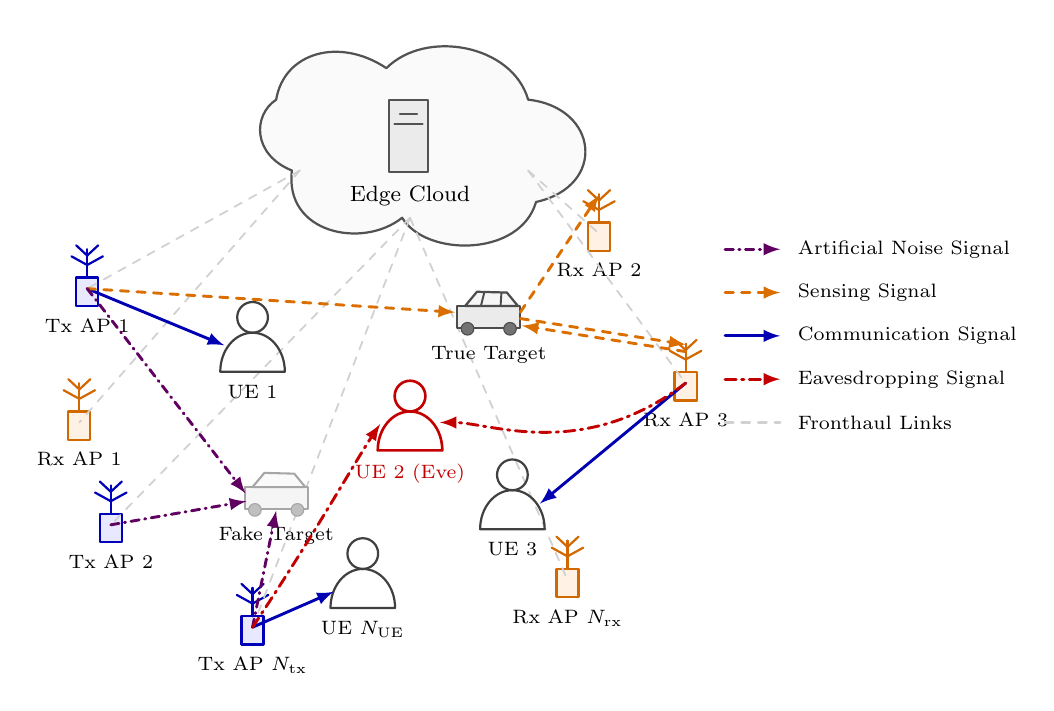
\begin{tikzpicture}[x=1mm,y=1mm,>=latex,font=\scriptsize,line cap=round,line join=round]
\colorlet{txc}{blue!72!black}
\colorlet{rxc}{orange!82!black}
\colorlet{commc}{blue!70!black}
\colorlet{sensc}{orange!86!black}
\colorlet{anc}{violet!75!black}
\colorlet{evec}{red!76!black}
\colorlet{cloudc}{black!68}
\colorlet{linkc}{black!18}

\tikzset{
    fronthaul/.style={linkc, dashed, line width=0.65pt},
    comm/.style={commc, line width=1.05pt, -latex},
    sensing/.style={sensc, dashed, line width=1.05pt, -latex},
    an/.style={anc, dash dot, line width=1.05pt, -latex},
    eve/.style={evec, dash pattern=on 4pt off 2pt on 0.8pt off 2pt, line width=1.05pt, -latex},
    label/.style={align=center, text=black}
}

% Edge cloud and fronthaul links.
\draw[cloudc, line width=0.8pt, fill=black!2]
    (31,62) .. controls (32,68) and (39,70) .. (45,66)
    .. controls (50,71) and (61,69) .. (63,62)
    .. controls (72,61) and (73,51) .. (64,49)
    .. controls (62,42) and (50,42) .. (47,47)
    .. controls (42,43) and (32,45) .. (33,53)
    .. controls (28,55) and (28,60) .. cycle;
\draw[cloudc, fill=black!8, line width=0.7pt] (45.3,52.8) rectangle (50.3,62.0);
\draw[cloudc, line width=0.7pt] (46.7,60.2) -- (48.9,60.2);
\draw[cloudc, line width=0.7pt] (46.0,58.9) -- (49.6,58.9);
\node[label, font=\footnotesize] at (48,49.8) {Edge Cloud};

\coordinate (cloudL) at (34,53);
\coordinate (cloudM) at (48,47);
\coordinate (cloudR) at (63,53);

% AP icon helper: radio head, mast, and antenna.
\def\TxAP#1#2#3{%
    \coordinate (#1) at (#2,#3);
    \draw[txc, fill=blue!9, line width=0.8pt] ($(#1)+(-1.4,-2.2)$) rectangle ($(#1)+(1.4,1.4)$);
    \draw[txc, line width=0.8pt] ($(#1)+(0,1.4)$) -- ($(#1)+(0,5.0)$);
    \draw[txc, line width=0.8pt] ($(#1)+(0,3.0)$) -- ($(#1)+(-2.0,4.1)$);
    \draw[txc, line width=0.8pt] ($(#1)+(0,3.0)$) -- ($(#1)+(2.0,4.1)$);
    \draw[txc, line width=0.8pt] ($(#1)+(0,4.2)$) -- ($(#1)+(-1.4,5.5)$);
    \draw[txc, line width=0.8pt] ($(#1)+(0,4.2)$) -- ($(#1)+(1.4,5.5)$);
}
\def\RxAP#1#2#3{%
    \coordinate (#1) at (#2,#3);
    \draw[rxc, fill=orange!11, line width=0.8pt] ($(#1)+(-1.4,-2.2)$) rectangle ($(#1)+(1.4,1.4)$);
    \draw[rxc, line width=0.8pt] ($(#1)+(0,1.4)$) -- ($(#1)+(0,5.0)$);
    \draw[rxc, line width=0.8pt] ($(#1)+(0,3.0)$) -- ($(#1)+(-2.0,4.1)$);
    \draw[rxc, line width=0.8pt] ($(#1)+(0,3.0)$) -- ($(#1)+(2.0,4.1)$);
    \draw[rxc, line width=0.8pt] ($(#1)+(0,4.2)$) -- ($(#1)+(-1.4,5.5)$);
    \draw[rxc, line width=0.8pt] ($(#1)+(0,4.2)$) -- ($(#1)+(1.4,5.5)$);
}
\def\UEIcon#1#2#3{%
    \draw[#2, line width=#3] ($(#1)+(0,4.35)$) circle (1.95);
    \draw[#2, line width=#3] ($(#1)+(-4.1,-2.55)$) -- ($(#1)+(4.1,-2.55)$)
        arc[start angle=0,end angle=180,x radius=4.1,y radius=4.95] -- cycle;
}

% Node icons.
\TxAP{tx1}{7}{38}
\node[label, anchor=north] at (tx1 |- 4,35.4) {Tx AP 1};
\RxAP{rx1}{6}{21}
\node[label, anchor=north] at (rx1 |- 4,18.4) {Rx AP 1};
\TxAP{tx2}{10}{8}
\node[label, anchor=north] at (tx2 |- 4,5.4) {Tx AP 2};
\TxAP{txn}{28}{-5}
\node[label, anchor=north] at (txn |- 4,-7.6) {Tx AP $N_{\mathrm{tx}}$};

\RxAP{rx2}{72}{45}
\node[label, anchor=north] at (rx2 |- 4,42.4) {Rx AP 2};
\RxAP{rx3}{83}{26}
\node[label, anchor=north] at (rx3 |- 4,23.4) {Rx AP 3};
\RxAP{rxn}{68}{1}
\node[label, anchor=north] at (rxn |- 4,-1.6) {Rx AP $N_{\mathrm{rx}}$};

\draw[fronthaul] (cloudL) -- (tx1);
\draw[fronthaul] (cloudL) -- (rx1);
\draw[fronthaul] (cloudM) -- (tx2);
\draw[fronthaul] (cloudM) -- (txn);
\draw[fronthaul] (cloudR) -- (rx2);
\draw[fronthaul] (cloudR) -- (rx3);
\draw[fronthaul] (cloudM) -- (rxn);

% Users.
\coordinate (u1) at (28,30);
\UEIcon{u1}{black!75}{0.8pt}
\node[label, anchor=north] at ($(u1)+(0,-3.0)$) {UE 1};

\coordinate (un) at (42,0);
\UEIcon{un}{black!75}{0.8pt}
\node[label, anchor=north] at ($(un)+(0,-3.0)$) {UE $N_{\mathrm{UE}}$};

\coordinate (u3) at (61,10);
\UEIcon{u3}{black!75}{0.8pt}
\node[label, anchor=north] at ($(u3)+(0,-3.0)$) {UE 3};

\coordinate (eveu) at (48,20);
\UEIcon{eveu}{evec}{0.95pt}
\node[label, text=evec, anchor=north] at ($(eveu)+(0,-3.0)$) {UE 2 (Eve)};

% Targets.
\coordinate (target) at (58,34);
\draw[black!70, fill=black!8, line width=0.8pt] ($(target)+(-4,-1.0)$) rectangle ($(target)+(4,1.8)$);
\draw[black!70, fill=black!4, line width=0.8pt] ($(target)+(-3.0,1.8)$)
    -- ($(target)+(-1.5,3.6)$) -- ($(target)+(2.3,3.5)$)
    -- ($(target)+(3.7,1.8)$) -- cycle;
\draw[black!70, line width=0.7pt] ($(target)+(-1.0,1.8)$) -- ($(target)+(-0.6,3.4)$);
\draw[black!70, line width=0.7pt] ($(target)+(1.5,1.8)$) -- ($(target)+(1.6,3.4)$);
\draw[black!70, fill=black!55] ($(target)+(-2.7,-1.1)$) circle (0.8);
\draw[black!70, fill=black!55] ($(target)+(2.7,-1.1)$) circle (0.8);
\node[label, anchor=north] at ($(target)+(0,-2.1)$) {True Target};

\coordinate (fake) at (31,11);
\draw[black!35, fill=black!4, line width=0.75pt] ($(fake)+(-4,-1.0)$) rectangle ($(fake)+(4,1.8)$);
\draw[black!35, fill=black!2, line width=0.75pt] ($(fake)+(-3.0,1.8)$)
    -- ($(fake)+(-1.5,3.6)$) -- ($(fake)+(2.3,3.5)$)
    -- ($(fake)+(3.7,1.8)$) -- cycle;
\draw[black!35, fill=black!25] ($(fake)+(-2.7,-1.1)$) circle (0.8);
\draw[black!35, fill=black!25] ($(fake)+(2.7,-1.1)$) circle (0.8);
\node[label, anchor=north] at ($(fake)+(0,-2.1)$) {Fake Target};

% Signal paths.
\draw[comm] (tx1) -- ($(u1)+(-3.6,0.8)$);
\draw[comm] (txn) -- ($(un)+(-3.7,-0.5)$);
\draw[comm] (rx3) -- ($(u3)+(3.5,0.7)$);

\draw[sensing] (tx1) -- ($(target)+(-4.3,1.0)$);
\draw[sensing] ($(target)+(4.0,1.0)$) -- ($(rx2)+(0,4.9)$);
\draw[sensing] ($(target)+(4.0,0.2)$) -- ($(rx3)+(0,4.9)$);
\draw[sensing] ($(rx3)+(0,4.0)$) -- ($(target)+(4.2,-0.7)$);

\draw[an] (tx1) -- ($(fake)+(-3.9,1.0)$);
\draw[an] (tx2) -- ($(fake)+(-3.8,0.0)$);
\draw[an] (txn) -- ($(fake)+(0.0,-1.2)$);

\draw[eve] (txn) .. controls (36,7) and (41,16) .. ($(eveu)+(-3.8,0.8)$);
\draw[eve] (rx3) .. controls (70,16) and (58,21) .. ($(eveu)+(3.8,1.0)$);

% Legend.
\draw[an] (88,43) -- (95,43);
\node[anchor=west] at (96,43) {Artificial Noise Signal};
\draw[sensing] (88,37.5) -- (95,37.5);
\node[anchor=west] at (96,37.5) {Sensing Signal};
\draw[comm] (88,32) -- (95,32);
\node[anchor=west] at (96,32) {Communication Signal};
\draw[eve] (88,26.5) -- (95,26.5);
\node[anchor=west] at (96,26.5) {Eavesdropping Signal};
\draw[fronthaul, line width=0.9pt] (88,21) -- (95,21);
\node[anchor=west] at (96,21) {Fronthaul Links};
\end{tikzpicture}
}
    \caption{System model of the CF-mMIMO ISAC network.}
    \label{fig:layout}
\end{figure}

\subsection{Multi-Static CF-mMIMO ISAC Model}
As illustrated in Fig.~\ref{fig:layout}, we consider a downlink multi-static CF-mMIMO ISAC network with $N_{\mathrm{tx}}$ transmitting APs, $N_{\mathrm{rx}}$ receiving APs, and $N_{\mathrm{UE}}$ multi-antenna users. Each transmitting AP employs an $M_{\mathrm{tx}}$-element half-wavelength uniform linear array (ULA), and each user has $M_{\mathrm{UE}}$ antennas. The APs are coordinated by a central processor to serve users and illuminate a point target. One served user may behave as an internal adversary and infer target information from received signals. Hence, the signal emitted by AP $k$ at time index $n$ is
\begin{equation}
\mathbf{x}_k[n]=\sum_{i=1}^{N_{\mathrm{UE}}}\mathbf{w}_{i,k}s_i[n]+\mathbf{w}_{t,k}s_t[n],
\label{eq:xk}
\end{equation}
where $\mathbf{w}_{i,k}\in\mathbb{C}^{M_{\mathrm{tx}}\times 1}$ is the beam for user $i$ and $\mathbf{w}_{t,k}\in\mathbb{C}^{M_{\mathrm{tx}}\times 1}$ is the sensing beam.
The symbols $s_i[n]$ and $s_t[n]$ are independent and unit-power normalized.
Following the standard CF-mMIMO model \cite{ngo2017cellfree}, the AP-user channel $\mathbf{H}_{i,k}\in\mathbb{C}^{M_{\mathrm{UE}}\times M_{\mathrm{tx}}}$ is modeled as $\mathbf{H}_{i,k}=\sqrt{\beta_{i,k}}\,\mathbf{G}_{i,k}$, where $\mathbf{G}_{i,k}$ has i.i.d. $\mathcal{CN}(0,1)$ entries and $\beta_{i,k}$ is the large-scale fading coefficient. The received signal at user $i$ is $\mathbf{y}_i[n]=\sum_k\mathbf{H}_{i,k}\mathbf{x}_k[n]+\mathbf{n}_i[n]$ with additive noise $\mathbf{n}_i[n]\sim\mathcal{CN}(\mathbf{0},\sigma_i^2\mathbf{I})$. User $i$ applies a unit-norm linear combiner $\mathbf{u}_i\in\mathbb{C}^{M_{\mathrm{UE}}\times 1}$ ($\|\mathbf{u}_i\|=1$), yielding the downlink SINR
\begin{equation}
\gamma_i=
\frac{\left|\sum_{k}\mathbf{u}_i^H\mathbf{H}_{i,k}\mathbf{w}_{i,k}\right|^2}{\sum_{j\neq i}\left|\sum_{k}\mathbf{u}_i^H\mathbf{H}_{i,k}\mathbf{w}_{j,k}\right|^2+\left|\sum_{k}\mathbf{u}_i^H\mathbf{H}_{i,k}\mathbf{w}_{t,k}\right|^2+\sigma_i^2},
\label{eq:sinr-user}
\end{equation}
where $\mathbf{w}_{t,k}$ contributes interference to legitimate users.

For multi-static sensing, transmit AP $k$ illuminates the target at angle $\phi_k$ with ULA steering vector $\mathbf{a}(\phi)=[1,e^{j\pi\sin\phi},\ldots,e^{j(M_{\mathrm{tx}}-1)\pi\sin\phi}]^T$, where $\phi$ denotes an arbitrary angle. Each receive AP $r$ captures the reflected echo via a LoS-dominated bistatic path with scattering coefficient $\alpha_{r,k}\sim\mathcal{CN}(0,\xi_{r,k}^2)$ and bistatic path gain $g_{r,k}=\lambda_c^2/[(4\pi)^3 d_{t,k}^2 d_{t,r}^2]$, where $\lambda_c$ is the carrier wavelength, and $d_{t,k}$ and $d_{t,r}$ are the target distances to transmitting AP $k$ and receiving AP $r$, respectively. Defining $\mathbf{W}_k=[\mathbf{w}_{1,k},\ldots,\mathbf{w}_{N_{\mathrm{UE}},k},\mathbf{w}_{t,k}]$ and averaging over independent scattering coefficients and normalized symbols yields the multi-static sensing SNR
\begin{equation}
\gamma_t=\sum_{k=1}^{N_{\mathrm{tx}}}c_k\left\|\mathbf{a}^H(\phi_k)\mathbf{W}_k\right\|_F^2,\quad c_k=\frac{\sum_{r}\xi_{r,k}^2 g_{r,k}}{N_{\mathrm{rx}}\sigma_n^2},
\label{eq:snr-sensing}
\end{equation}
where $\sigma_n^2$ is the per-antenna noise power at each receive AP.

\subsection{Internal Beampattern-Reconstruction Threat}
\label{subsec:threat}
One served user, indexed by $a$, is treated as an honest-but-curious internal adversary. It follows the communication protocol but exploits its received signals for sensing inference. Specifically, as a legitimate user, it has a synchronized downlink connection, knows its own pilots/data symbols, and can estimate the AP-user channel on its own link via least-squares, yielding an imperfect estimate $\widehat{\mathbf{H}}_{a,k}=\mathbf{H}_{a,k}+\boldsymbol{\varepsilon}_{a,k}$, where $\boldsymbol{\varepsilon}_{a,k}\in\mathbb{C}^{M_{\mathrm{UE}}\times M_{\mathrm{tx}}}$ collects the AP-wise CSI errors. It also knows its receive combiner $\mathbf{u}_a$ and the transmit-AP positions. However, applying $\mathbf{u}_a$ would collapse the multi-antenna structure required by the reconstruction, so the adversary operates on the raw multi-antenna samples before combining. This capability is stronger than that of an external eavesdropper because the adversary is embedded in the served-user set and observes AP transmissions through legitimate channels.

Following the privacy-assessment model of \cite{dasilva2023multistaticcf}, and assuming AP-wise resource separation via orthogonal pilots that lets the adversary isolate the contribution of each transmitting AP, the adversary first identifies the non-self transmit component
\begin{equation}
\widetilde{\mathbf{x}}_k[n]=\sum_{j\neq a}\mathbf{w}_{j,k}s_j[n]+\mathbf{w}_{t,k}s_t[n],
\end{equation}
whose received version at the adversary, after subtraction of the known self-contribution, is $\widetilde{\mathbf{y}}_{a,k}[n]=\mathbf{H}_{a,k}\widetilde{\mathbf{x}}_k[n]+\mathbf{n}_{a,k}[n]$, with $\mathbf{n}_{a,k}[n]\sim\mathcal{CN}(\mathbf{0},\sigma_a^2\mathbf{I})$. The adversary then applies an expectation-maximization (EM) routine that absorbs the residual CSI error via a heavy-tailed Student's-$t$ prior \cite{dasilva2023multistaticcf}, yielding an estimate $\widehat{\mathbf{x}}_k[n]\approx\widetilde{\mathbf{x}}_k[n]$. It then forms the AP-dependent reconstructed beampattern
\begin{equation}
\widehat{B}_k(\theta)=\left|\mathbf{a}^H(\theta)\widehat{\mathbf{x}}_k[n]\right|^2,
\label{eq:beampattern}
\end{equation}
where $\theta$ denotes the search angle scanned by the adversary.
The dominant directions of $\{\widehat{B}_k(\theta)\}_k$ are then fused across APs on a search grid to infer the target position. This letter focuses on designing the active defense that preserves legitimate communication and sensing while forcing $\widehat{B}_k(\theta)$ to contain a misleading fake peak.

\section{Proposed Design}
\subsection{Asymmetric Null-Space AN Construction}
\label{subsec:asym}

To defend against the reconstructed-beampattern leakage, we augment the transmit signal at AP $k$ as
\begin{equation}
\mathbf{x}_k[n]=\sum_{i=1}^{N_{\mathrm{UE}}}\mathbf{w}_{i,k}s_i[n]+\mathbf{w}_{t,k}s_t[n]+\mathbf{z}_ks_z[n],
\label{eq:xk-an}
\end{equation}
where $\mathbf{z}_k\in\mathbb{C}^{M_{\mathrm{tx}}\times 1}$ is the AN beam and $s_z[n]$ is a unit-power AN symbol independent of $\{s_i[n],s_t[n]\}$. The legitimate-user SINR becomes \eqref{eq:sinr-user} augmented with the AN term $|\sum_k\mathbf{u}_i^H\mathbf{H}_{i,k}\mathbf{z}_k|^2$ in the denominator.

As Fig.~\ref{fig:asymmetry} illustrates, legitimate detection of user $i$ takes place after the receive combiner $\mathbf{u}_i$, so the effective AP-user channel reduces to the row vector $\mathbf{g}_{i,k}^H\triangleq\mathbf{u}_i^H\mathbf{H}_{i,k}\in\mathbb{C}^{1\times M_{\mathrm{tx}}}$, whose inner product with any transmit vector collapses the $M_{\mathrm{UE}}$-dim raw observation to a one-dimensional decision statistic. In contrast, the internal adversary's EM-based reconstruction operates on the raw multi-antenna observation and sees the full $M_{\mathrm{UE}}\times M_{\mathrm{tx}}$ channel $\mathbf{H}_{i,k}$. Applying its own combiner $\mathbf{u}_a^H$ would compress each time sample into a single scalar, leaving the resulting linear system underdetermined for recovering the $M_{\mathrm{tx}}$-dimensional transmit vector $\widetilde{\mathbf{x}}_k[n]$, so the adversary must retain the raw $M_{\mathrm{UE}}$-dimensional observation as input to its EM routine. We therefore impose the effective-channel nulling condition $\mathbf{g}_{i,k}^H\mathbf{z}_k=0,\ \forall i,k$, which is strictly weaker than the conventional null-space condition $\mathbf{H}_{i,k}\mathbf{z}_k=\mathbf{0}$ adopted by classical physical layer security AN designs.

The feasible AN subspace at AP $k$ is consequently the null space of $[\mathbf{g}_{1,k},\ldots,\mathbf{g}_{N_{\mathrm{UE}},k}]^H$, whose dimension is $M_{\mathrm{tx}}-\operatorname{rank}([\mathbf{g}_{1,k},\ldots,\mathbf{g}_{N_{\mathrm{UE}},k}]^H)$. For effective channels with $M_{\mathrm{tx}}\ge N_{\mathrm{UE}}$, this dimension reduces to $M_{\mathrm{tx}}-N_{\mathrm{UE}}$. By contrast, conventional null-space AN based on $\mathbf{H}_{i,k}\mathbf{z}_k=\mathbf{0}$ has dimension $M_{\mathrm{tx}}-\operatorname{rank}([\mathbf{H}_{1,k}^T,\ldots,\mathbf{H}_{N_{\mathrm{UE}},k}^T]^T)$, which reduces to $\max\{M_{\mathrm{tx}}-N_{\mathrm{UE}}M_{\mathrm{UE}},\,0\}$. Thus, our scheme preserves the transmit directions that are discarded by legitimate combining but remain present in the raw samples that drive the adversary's reconstruction. As a result, the asymmetric AN subspace is non-empty whenever $M_{\mathrm{tx}}>N_{\mathrm{UE}}$, a substantially milder requirement than that of conventional null-space AN.

\subsection{Fake-Peak AN Beam Design}
Within the asymmetric subspace identified in Section~\ref{subsec:asym}, we further concentrate the AN energy along a preset fake direction $\phi_{\mathrm{fake},k}\neq\phi_k$, so that the adversary's per-AP reconstructed beampattern $\widehat{B}_k(\theta)$ contains a deceptive peak whose multi-AP fusion points to a misleading target location. The CPU is assumed to have perfect CSI of the legitimate links for beam design, while CSI errors on the adversary side are absorbed into the EM model of \cite{dasilva2023multistaticcf}. Let $\Gamma_{\mathrm{comm}}$ denote the minimum required user SINR, $P_T$ the per-AP transmit-power budget, and $\rho$ the required fake-peak strength ratio relative to the true-direction beam. The resulting secure beam design is formulated as
\begin{subequations}
\begin{align}
\max_{\{\mathbf{W}_k,\mathbf{z}_k,\mathbf{u}_i\}} \quad & \sum_{k=1}^{N_{\mathrm{tx}}}c_k\left\|\mathbf{a}^H(\phi_k)\mathbf{W}_k\right\|_F^2 \label{prob:obj}\\
\text{s.t.}\quad & \gamma_i\ge \Gamma_{\mathrm{comm}},\quad \forall i, \label{prob:sinr}\\
& \textstyle\sum_{i=1}^{N_{\mathrm{UE}}}\|\mathbf{w}_{i,k}\|^2+\|\mathbf{w}_{t,k}\|^2+\|\mathbf{z}_k\|^2\le P_T,\quad \forall k, \label{prob:power}\\
& \mathbf{u}_i^H\mathbf{H}_{i,k}\mathbf{z}_k=0,\quad \forall i,\forall k, \label{prob:null}\\
& \left|\mathbf{a}^H(\phi_{\mathrm{fake},k})\mathbf{z}_k\right|^2 \ge \rho\left\|\mathbf{a}^H(\phi_k)\mathbf{W}_k\right\|_F^2,\quad \forall k. \label{prob:fake}
\end{align}
\end{subequations}
Constraint \eqref{prob:sinr} enforces the communication QoS, \eqref{prob:power} caps the per-AP transmit power, \eqref{prob:null} confines $\mathbf{z}_k$ to the asymmetric AN subspace of Section~\ref{subsec:asym}, and \eqref{prob:fake} forces the AN to form a fake peak. The sensing objective counts only the useful beams for the true target, treating the AN waveform as a known deception signal rather than as part of the desired return. Problem \eqref{prob:obj}--\eqref{prob:fake} is non-convex, and is solved by alternating between a CCCP transmit update and an MMSE receive-combiner update.

\begin{figure}[t]
    \centering
    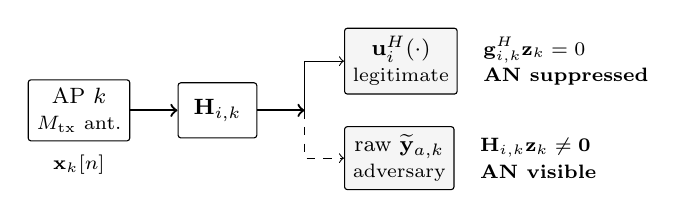
\begin{tikzpicture}[font=\footnotesize,
        block/.style={draw, rounded corners=1pt, minimum height=7mm, inner sep=3pt, align=center},
        node distance=3mm and 6mm]
        \node[block, minimum width=12mm] (TX) {AP $k$\\\scriptsize $M_{\mathrm{tx}}$ ant.};
        \node[below=0.5mm of TX, align=center] {\scriptsize $\mathbf{x}_k[n]$};
        \node[block, right=6mm of TX, minimum width=10mm] (H) {$\mathbf{H}_{i,k}$};
        \coordinate (br) at ($(H.east)+(6mm,0)$);
        \node[block, above right=2mm and 5mm of br, minimum width=11mm, fill=black!4] (U)
            {$\mathbf{u}_i^H(\cdot)$\\\scriptsize legitimate};
        \node[right=2mm of U, align=left] {\scriptsize $\mathbf{g}_{i,k}^H\mathbf{z}_k=0$\\\scriptsize\textbf{AN suppressed}};
        \node[block, below right=2mm and 5mm of br, minimum width=11mm, fill=black!4] (R)
            {raw $\widetilde{\mathbf{y}}_{a,k}$\\\scriptsize adversary};
        \node[right=2mm of R, align=left] {\scriptsize $\mathbf{H}_{i,k}\mathbf{z}_k\neq\mathbf{0}$\\\scriptsize\textbf{AN visible}};
        \draw[->, thick] (TX) -- (H);
        \draw[->, thick] (H) -- (br);
        \draw[->] (br) |- (U);
        \draw[->, dashed] (br) |- (R);
    \end{tikzpicture}
    \caption{Effective- vs. raw-channel asymmetry exploited by the proposed AN.}
    \label{fig:asymmetry}
\end{figure}

\subsection{CCCP-MMSE Alternating Algorithm}
The proposed algorithm alternates two updates: a CCCP-based convex transmit update for fixed $\{\mathbf{u}_i\}$, and an MMSE update of $\{\mathbf{u}_i\}$ for fixed transmit beams. Let $\mathbf{W}\triangleq\{\mathbf{W}_k\}_{k=1}^{N_{\mathrm{tx}}}$ and $\mathbf{z}\triangleq\{\mathbf{z}_k\}_{k=1}^{N_{\mathrm{tx}}}$. Define $\mathbf{A}_k=\mathbf{a}(\phi_k)\mathbf{a}^H(\phi_k)$, $\mathbf{A}_{\mathrm{f},k}=\mathbf{a}(\phi_{\mathrm{fake},k})\mathbf{a}^H(\phi_{\mathrm{fake},k})$, and
\begin{equation}
    \begin{aligned}
    h_i(\mathbf{W})&={\textstyle\sum_k}\mathbf{u}_i^H\mathbf{H}_{i,k}\mathbf{w}_{i,k},\\
    \mathcal{I}_i(\mathbf{W},\mathbf{z})&={\textstyle\sum_{j\neq i}}\left|{\textstyle\sum_k}\mathbf{u}_i^H\mathbf{H}_{i,k}\mathbf{w}_{j,k}\right|^2
    +\left|{\textstyle\sum_k}\mathbf{u}_i^H\mathbf{H}_{i,k}\mathbf{w}_{t,k}\right|^2 \nonumber\\
    &\quad+\left|{\textstyle\sum_k}\mathbf{u}_i^H\mathbf{H}_{i,k}\mathbf{z}_k\right|^2+\sigma_i^2 .
    \end{aligned}
    \label{eq:auxiliary}
\end{equation}
Substituting these auxiliary symbols into \eqref{prob:obj}--\eqref{prob:fake} yields the fixed-combiner transmit-side subproblem
\begin{subequations}\label{eq:tx-orig}
\begin{align}
\max_{\{\mathbf{w}_{i,k},\mathbf{w}_{t,k},\mathbf{z}_k\}}\ & \sum_{k}c_k\mathrm{Tr}(\mathbf{W}_k^H\mathbf{A}_k\mathbf{W}_k)\\
\text{s.t.}\ & \Gamma_{\mathrm{comm}}\mathcal{I}_i(\mathbf{W},\mathbf{z})-|h_i(\mathbf{W})|^2\le 0,\ \forall i,\\
& \eqref{prob:power},\ \eqref{prob:null},\\
& \rho\,\mathrm{Tr}(\mathbf{W}_k^H\mathbf{A}_k\mathbf{W}_k)-\mathbf{z}_k^H\mathbf{A}_{\mathrm{f},k}\mathbf{z}_k\le 0,\ \forall k,
\end{align}
\end{subequations}
which is non-convex because it maximizes a convex quadratic objective and contains convex quadratic terms with negative signs in the constraints. CCCP replaces the non-convex parts by first-order lower bounds at $(\mathbf{W}^{(v)},\mathbf{z}^{(v)})$, where $(v)$ indexes the CCCP iteration. For any Hermitian $\mathbf{A}\succeq 0$ and reference point $\boldsymbol{\xi}^{(v)}$,
\begin{equation}
\boldsymbol{\xi}^H\mathbf{A}\boldsymbol{\xi}\ge 2\Re\!\left\{(\mathbf{A}\boldsymbol{\xi}^{(v)})^H\boldsymbol{\xi}\right\}-(\boldsymbol{\xi}^{(v)})^H\mathbf{A}\boldsymbol{\xi}^{(v)}.
\label{eq:basiclb}
\end{equation}
Applying \eqref{eq:basiclb} column-wise gives
\begin{equation}
    \begin{aligned}
    \widetilde f_0&={\textstyle\sum_k} c_k\!\left(2\Re\{\mathrm{Tr}[(\mathbf{A}_k\mathbf{W}_k^{(v)})^H\mathbf{W}_k]\}\right. \nonumber\\
    &\quad\left.-\mathrm{Tr}[(\mathbf{W}_k^{(v)})^H\mathbf{A}_k\mathbf{W}_k^{(v)}]\right),\\
    \widetilde h_i&=2\Re\{(h_i(\mathbf{W}^{(v)}))^*h_i(\mathbf{W})\}-|h_i(\mathbf{W}^{(v)})|^2,\\
    \widetilde z_k&=2\Re\{(\mathbf{A}_{\mathrm{f},k}\mathbf{z}_k^{(v)})^H\mathbf{z}_k\}
    -(\mathbf{z}_k^{(v)})^H\mathbf{A}_{\mathrm{f},k}\mathbf{z}_k^{(v)} .
    \end{aligned}
    \label{eq:cccp-lb}
\end{equation}
The transmit update then solves the convex problem
\begin{subequations}\label{eq:tx-cvx}
\begin{align}
\max_{\{\mathbf{w}_{i,k},\mathbf{w}_{t,k},\mathbf{z}_k\}}\quad & \widetilde f_0\\
\text{s.t.}\quad & \Gamma_{\mathrm{comm}}\mathcal{I}_i(\mathbf{W},\mathbf{z})-\widetilde h_i\le 0,\ \forall i,\\
& \eqref{prob:power},\ \eqref{prob:null},\\
& \rho\,\mathrm{Tr}(\mathbf{W}_k^H\mathbf{A}_k\mathbf{W}_k)-\widetilde z_k\le 0,\ \forall k.
\end{align}
\end{subequations}
Here the objective function is affine, the SINR and fake-direction constraints are convex quadratic inequalities, and the null-space constraint is affine. Each CCCP iteration involves $\mathcal{O}(N_{\mathrm{tx}}M_{\mathrm{tx}}(N_{\mathrm{UE}}{+}2))$ variables and $\mathcal{O}(N_{\mathrm{tx}}{+}N_{\mathrm{UE}})$ constraints, and can be solved by standard convex solvers.

After each transmit update, each combiner is refreshed by the MMSE direction
\begin{equation}
\mathbf{u}_i=\frac{\mathbf{J}_i^{-1}\mathbf{v}_i}{\|\mathbf{J}_i^{-1}\mathbf{v}_i\|},\quad \mathbf{v}_i=\sum_{k}\mathbf{H}_{i,k}\mathbf{w}_{i,k},
\label{eq:mmse}
\end{equation}
where
\begin{equation}
    \begin{aligned}
    \mathbf{J}_i&={\textstyle\sum_{j\neq i}}\mathbf{q}_{i,j}\mathbf{q}_{i,j}^H+\mathbf{q}_{i,t}\mathbf{q}_{i,t}^H
    +\mathbf{q}_{i,z}\mathbf{q}_{i,z}^H+\sigma_i^2\mathbf{I},\\
    \mathbf{q}_{i,j}&={\textstyle\sum_k}\mathbf{H}_{i,k}\mathbf{w}_{j,k},\quad
    \mathbf{q}_{i,t}={\textstyle\sum_k}\mathbf{H}_{i,k}\mathbf{w}_{t,k},\\
    \mathbf{q}_{i,z}&={\textstyle\sum_k}\mathbf{H}_{i,k}\mathbf{z}_k.
    \end{aligned}
    \label{eq:Jv}
\end{equation}
The normalization enforces $\|\mathbf{u}_i\|=1$. Starting from a feasible point satisfying \eqref{prob:sinr}--\eqref{prob:fake}, the algorithm alternates between \eqref{eq:tx-cvx} and \eqref{eq:mmse} until the sensing objective changes by less than a prescribed tolerance. For fixed combiners, each CCCP transmit step improves a valid lower bound of the original objective. The overall alternating procedure is therefore run to a numerical stationary point.

\section{Simulation Results}
We consider a CF-mMIMO ISAC network with $N_{\mathrm{tx}}=8$ transmitting APs, $N_{\mathrm{rx}}=4$ receiving APs, and $N_{\mathrm{UE}}=2$ users, where each transmitting AP and each user is equipped with $M_{\mathrm{tx}}=M_{\mathrm{UE}}=16$ antennas. The carrier frequency is $1.9$ GHz, the per-AP transmit power budget is $P_T=50$ dBm, the user SINR target is $\Gamma_{\mathrm{comm}}=10$ dB, and the noise variances at both the users and the receiving APs are set to $\sigma_i^2=\sigma_n^2=-94$ dBm. The default target is at $(-75,75)$ m, users at $(\pm 50,\pm 50)$ m, receiving APs at $(\pm 150,\pm 150)$ m, and the fake target at $(5,-25)$ m. The AN-power ratio is defined as $\eta=\sum_k\|\mathbf{z}_k\|^2/\sum_k\!\left(\sum_{i=1}^{N_{\mathrm{UE}}}\|\mathbf{w}_{i,k}\|^2+\|\mathbf{w}_{t,k}\|^2+\|\mathbf{z}_k\|^2\right)$. All curves are averaged over $5000$ independent channel realizations. 

% As a remark on baselines, we compare against conventional joint sensing-communication (JSC) and isotropic Gaussian AN under the same threat model.

Let $\Theta\in\Omega\triangleq\{\theta_1,\ldots,\theta_{N_\theta}\}$ be the true target-direction random variable. We adopt a uniform prior $p_i\triangleq\Pr(\Theta=\theta_i)=1/N_\theta$, and take $\Omega$ as a uniform grid over $[-90^\circ,90^\circ]$ with $1^\circ$ resolution, i.e., $N_\theta=181$. The adversary's per-AP dominant direction inferred from \eqref{eq:beampattern} is
\begin{equation}
\Theta^p_k\triangleq\arg\max_{\theta\in\Omega}\widehat{B}_k(\theta),\quad k=1,\ldots,N_{\mathrm{tx}},
\label{eq:thetap-perap}
\end{equation}
with the transition $q^{(k)}_{j|i}\triangleq\Pr(\Theta^p_k=\theta_j\mid\Theta=\theta_i)$ estimated as the empirical frequency $\#\{\Theta^p_k=\theta_j\mid\Theta=\theta_i\}/R$ across the $R=500$ channel realizations. The per-AP directional mutual information then reads
\begin{equation}
I_k(\Theta;\Theta^p_k)=\sum_{i,j} p_i q^{(k)}_{j|i}\log\frac{q^{(k)}_{j|i}}{\sum_{\ell} p_\ell q^{(k)}_{j|\ell}},
\label{eq:mi-basic}
\end{equation}
and quantifies the directional leakage through AP $k$.

\begin{figure}[!t]
    \centering
    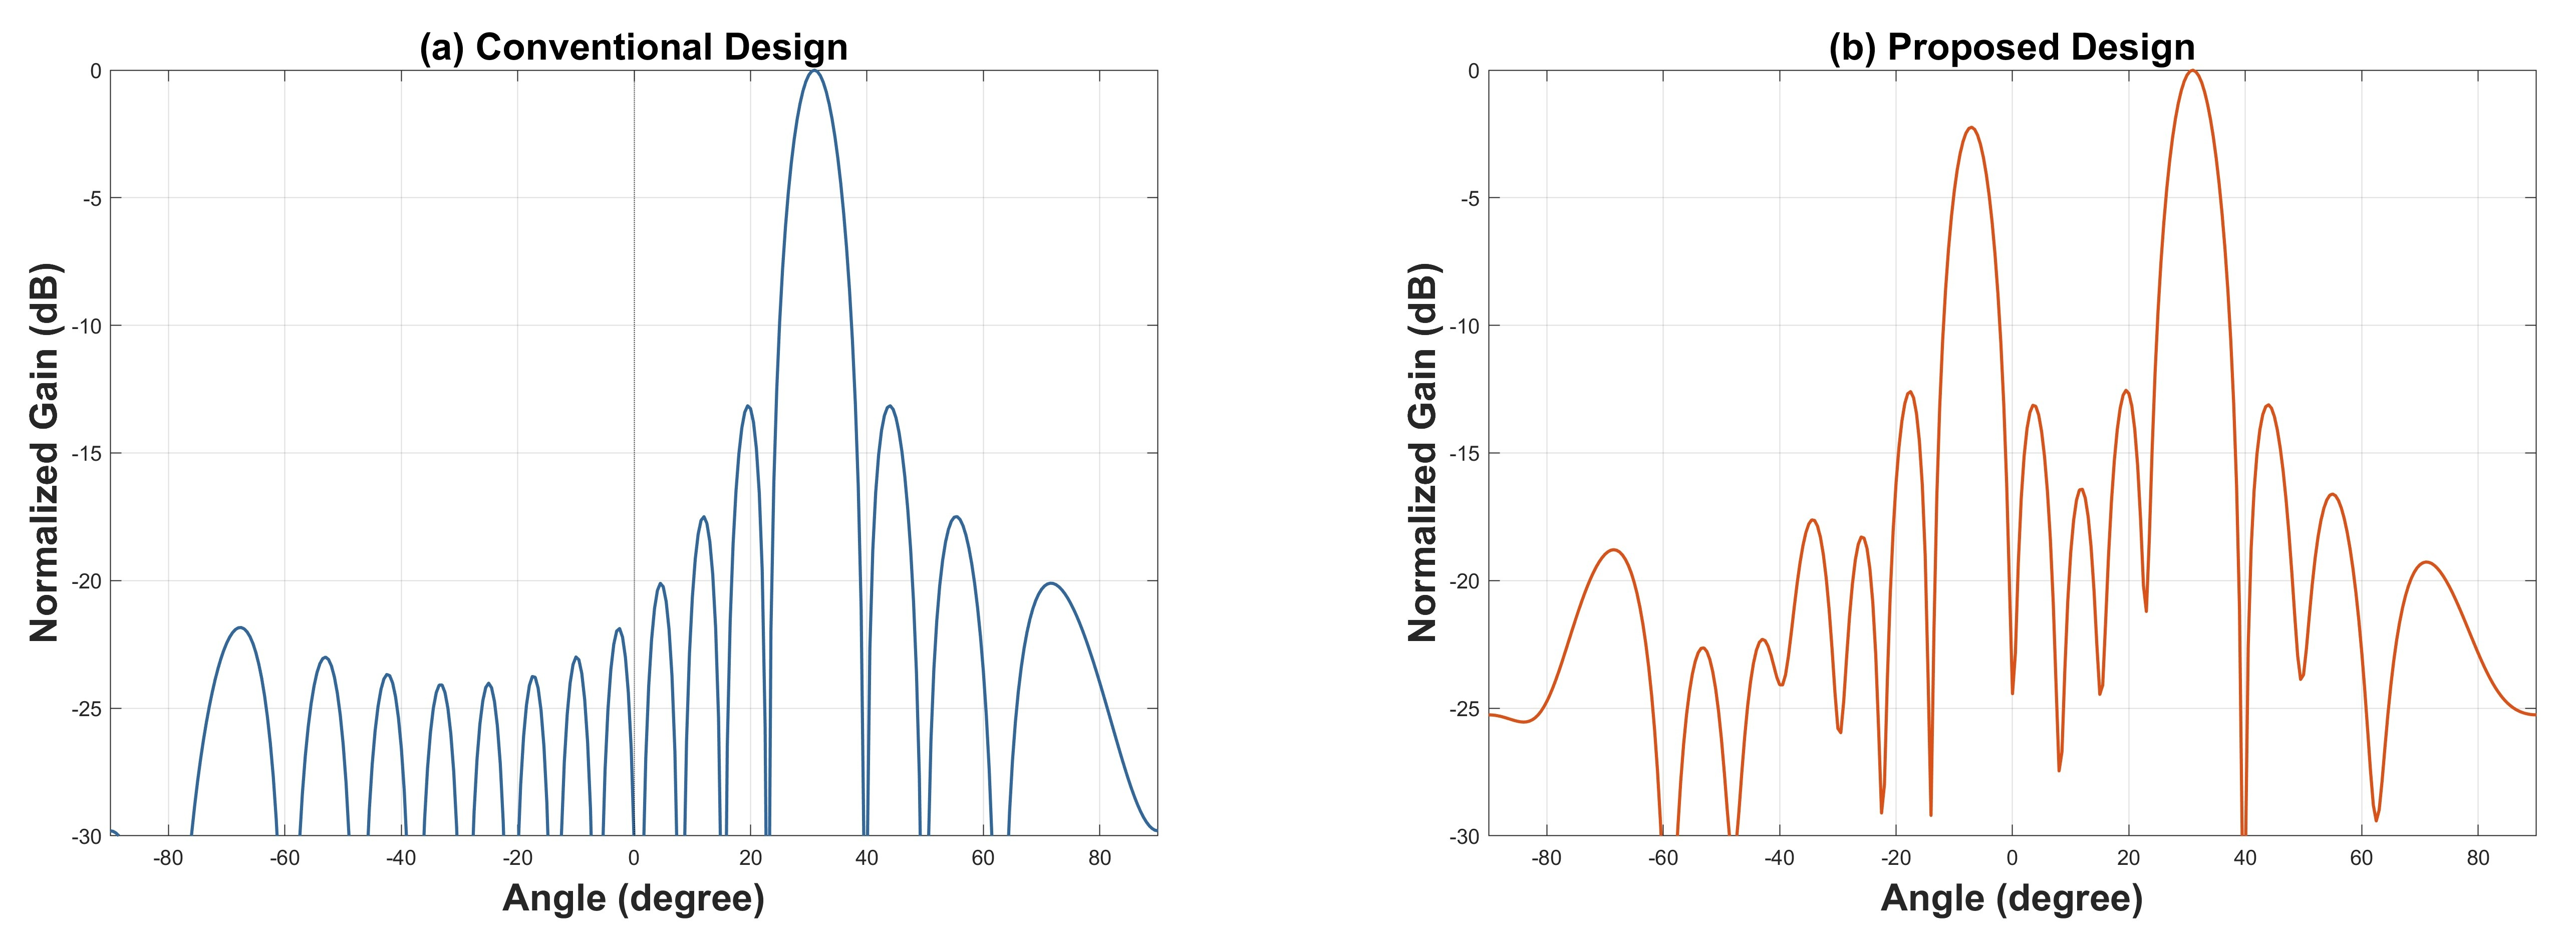
\includegraphics[width=0.98\columnwidth]{beampattern.jpg}
    \caption{Normalized transmit beampatterns at a representative transmitting AP.}
    \label{fig:beampatterns}
\end{figure}

Fig.~\ref{fig:beampatterns} compares the normalized transmit beampatterns at a representative transmitting AP. In Fig.~\ref{fig:beampatterns}(a), transmit energy concentrates around the true direction ($\approx 30^\circ$) with a single $0$~dB mainlobe and sidelobes below $-13$~dB, so the adversary locks onto the true direction almost deterministically. While in Fig.~\ref{fig:beampatterns}(b), the AN beam erects a second peak at the preset fake direction ($\approx -10^\circ$) that reaches the same $0$~dB level as the true-direction peak, a direct geometric consequence of the fake-peak constraint \eqref{prob:fake} with $\rho=1$. With two equal-height dominant lobes, the adversary can no longer concentrate on the true direction.

\begin{figure}[t]
    \centering
    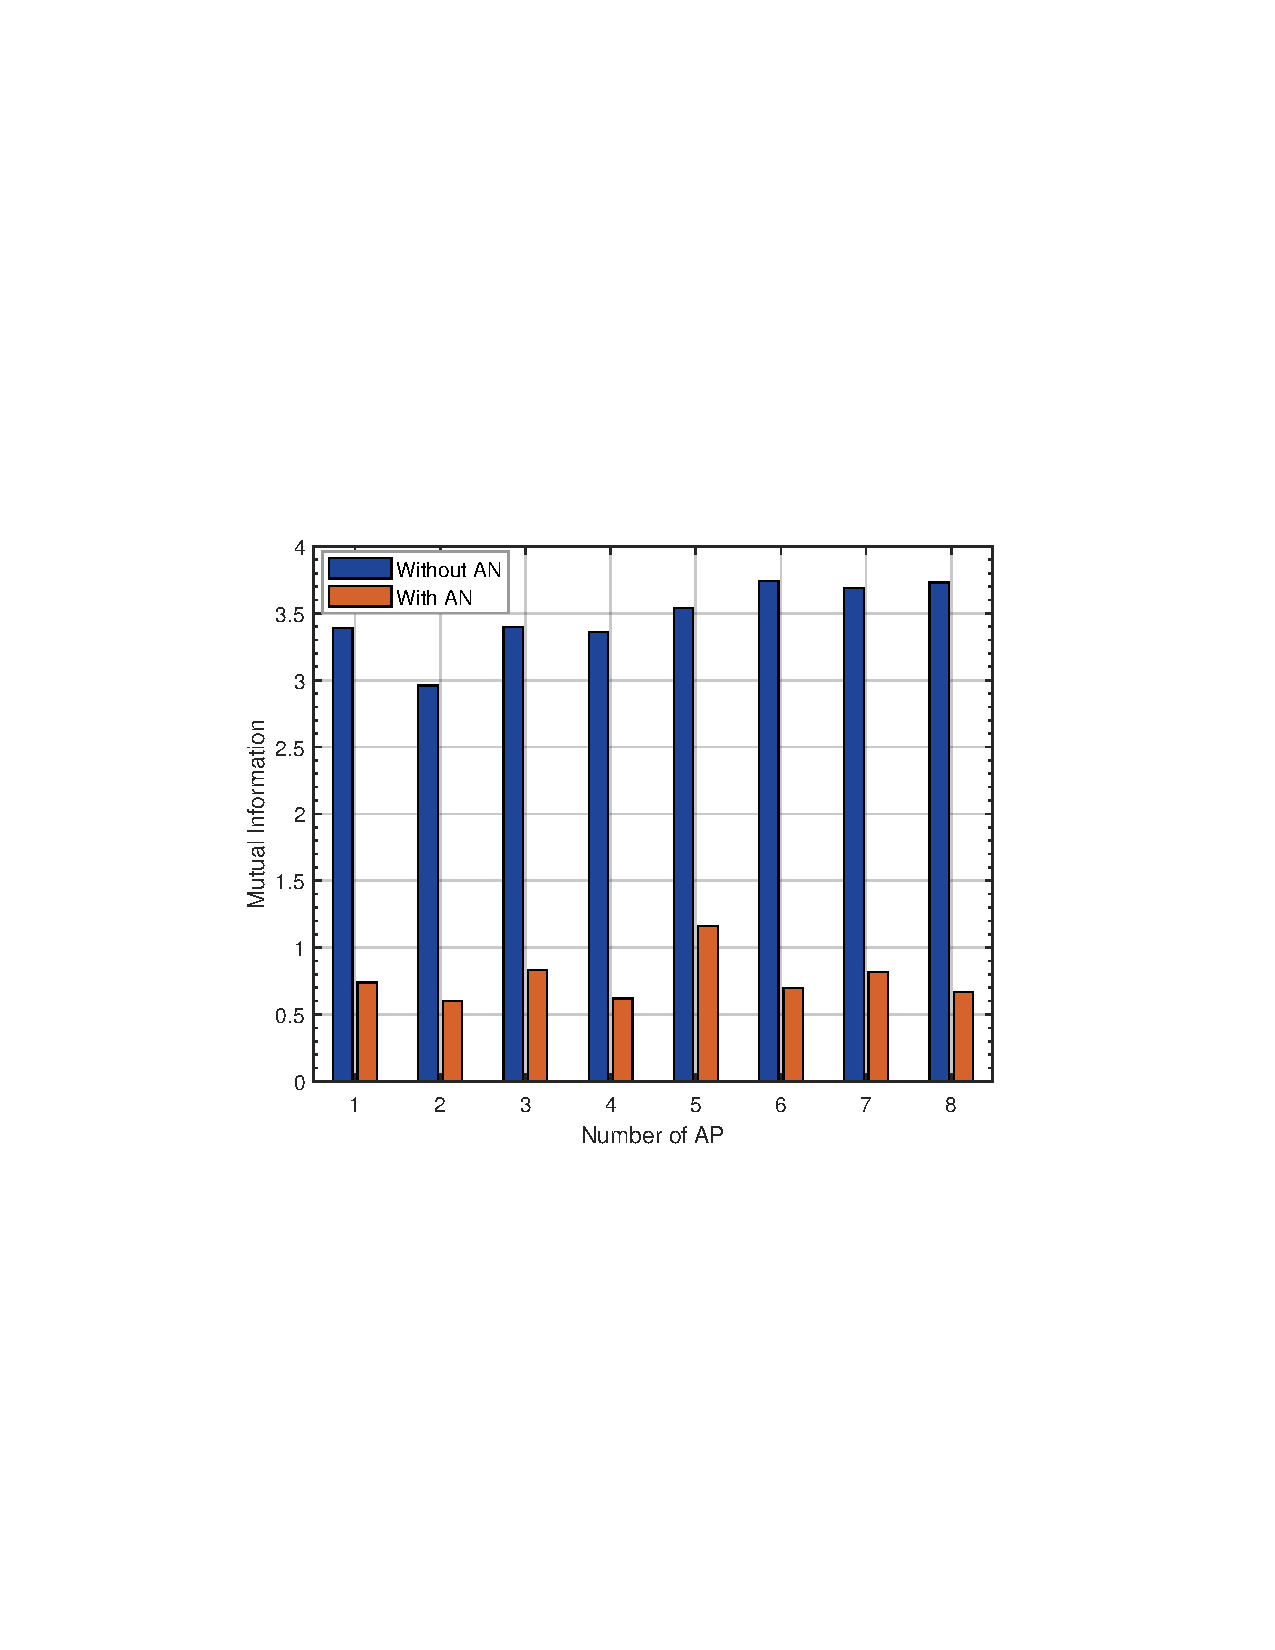
\includegraphics[width=0.8\columnwidth]{figure4.pdf}
    \caption{Per-AP directional mutual information $I_k(\Theta;\Theta^p_k)$ with and without the proposed AN.}
    \label{fig:mi}
\end{figure}

Fig.~\ref{fig:mi} reports $I_k$ in \eqref{eq:mi-basic} across all $N_{\mathrm{tx}}=8$ transmitting APs, with the prior-entropy ceiling $H(\Theta)=\log_2 N_\theta\approx 7.5$~bits. Under the conventional JSC design, $I_k$ ranges over $3.0$--$3.7$~bits ($\approx 40$--$50\%$ of $H(\Theta)$), confirming substantial true-direction information in the reconstructed beampattern. After the proposed AN is enabled, $I_k$ drops to $0.6$--$1.2$~bits, a $3$--$5\times$ reduction that is essentially uniform across the array. This uniform suppression is crucial because the adversary fuses per-AP dominant peaks (Sec.~\ref{subsec:threat}); a single un-suppressed AP would suffice to anchor the multi-AP fusion, so closing every leakage channel simultaneously is what makes the defense effective.

\begin{figure}[t]
    \centering
    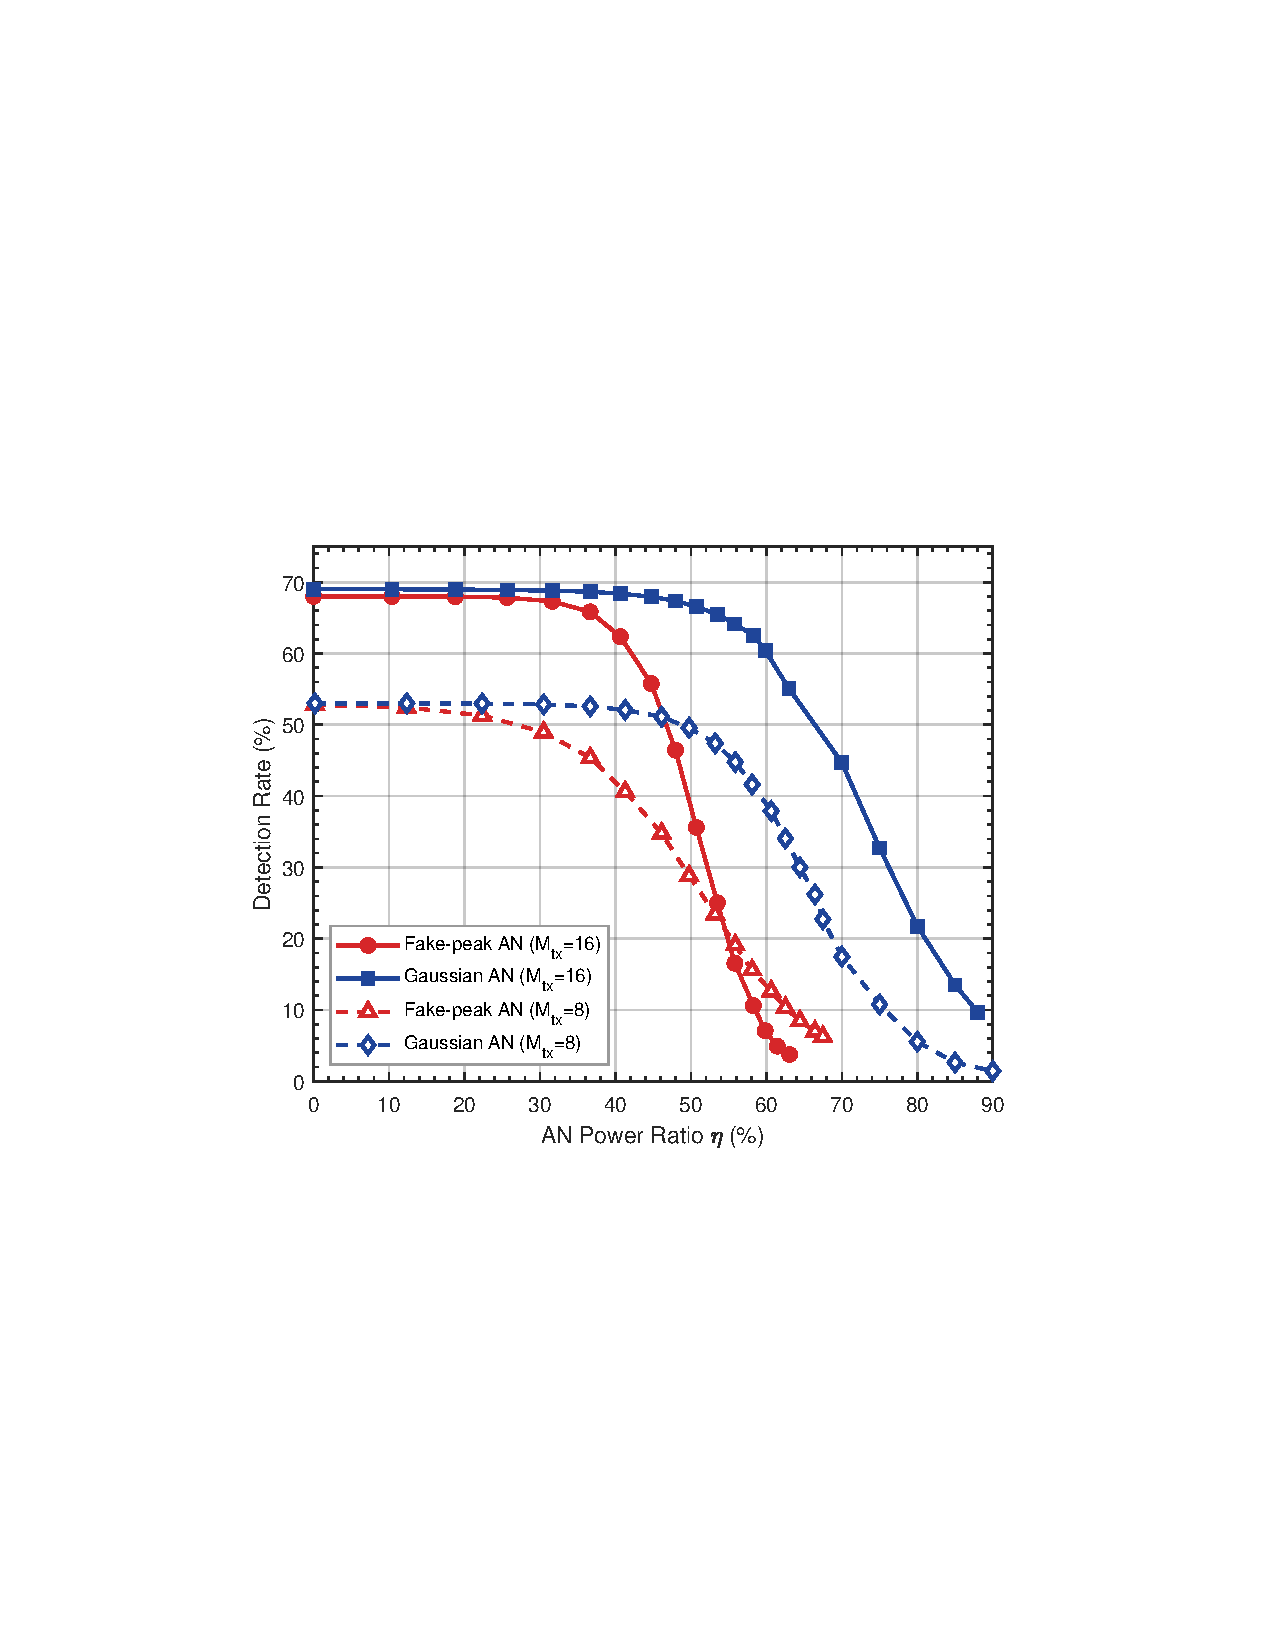
\includegraphics[width=0.8\columnwidth]{figure5.pdf}
    \caption{Adversary's detection rate versus AN-power ratio $\eta$ for fake-peak AN (red) and isotropic Gaussian AN (blue).}
    \label{fig:gauss-fake}
\end{figure}

Fig.~%
\ref{fig:gauss-fake} compares the proposed fake-peak AN with isotropic Gaussian AN over the entire AN-budget range.
The detection rate is defined as the empirical frequency that the adversary's per-AP $\arg\max$ $\Theta^p_k$ falls within $\pm 3^\circ$ of $\Theta$. At $M_{\mathrm{tx}}=16$, fake-peak AN drives the detection rate below $5\%$ already at $\eta\approx 0.59$, whereas Gaussian AN requires $\eta\approx 0.85$ to reach the same level, corresponding to an AN-budget saving of roughly $30$ percentage points. The gap widens at $M_{\mathrm{tx}}=8$, where fake-peak still achieves $\le 5\%$ detection at $\eta\approx 0.67$, while Gaussian AN saturates near $10\%$ even at $\eta=0.9$. The mechanism is geometric. The asymmetric AN subspace has dimension $M_{\mathrm{tx}}-N_{\mathrm{UE}}$ (Sec.~\ref{subsec:asym}), so Gaussian AN must dilute its power across $M_{\mathrm{tx}}-N_{\mathrm{UE}}$ basis directions and degrades rapidly as $M_{\mathrm{tx}}$ shrinks; the fake-peak design concentrates the entire AN budget on a single steered direction $\phi_{\mathrm{fake},k}$ and is therefore largely insensitive to the array DoF. Together with Fig.~\ref{fig:mi}, this confirms that the proposed scheme converts AN power into directional deception more efficiently than dispersion-based baselines.

\begin{figure}[t]
    \centering
    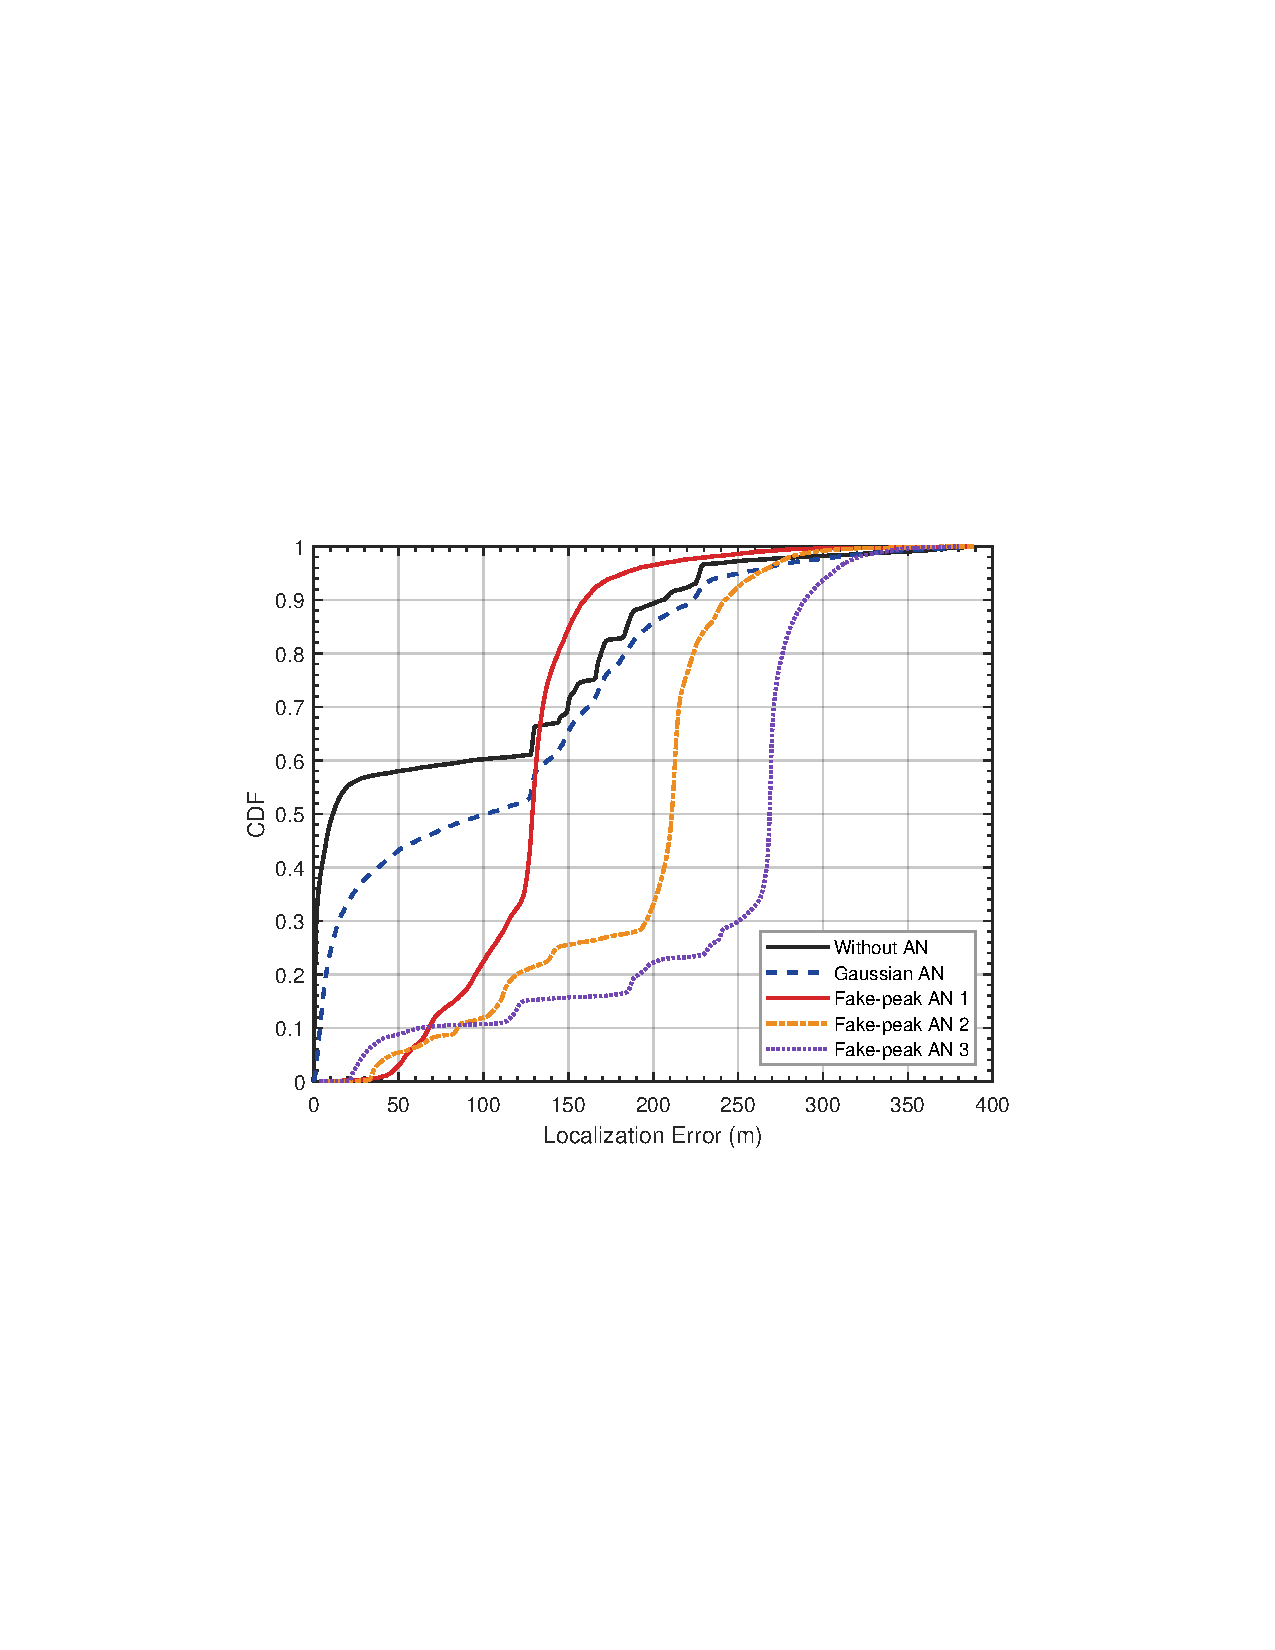
\includegraphics[width=0.8\columnwidth]{figure7.pdf}
    \caption{CDF of the adversary's localization error under different AN designs.}
    \label{fig:loc-error-cdf}
\end{figure}

\begin{figure}[t]
    \centering
    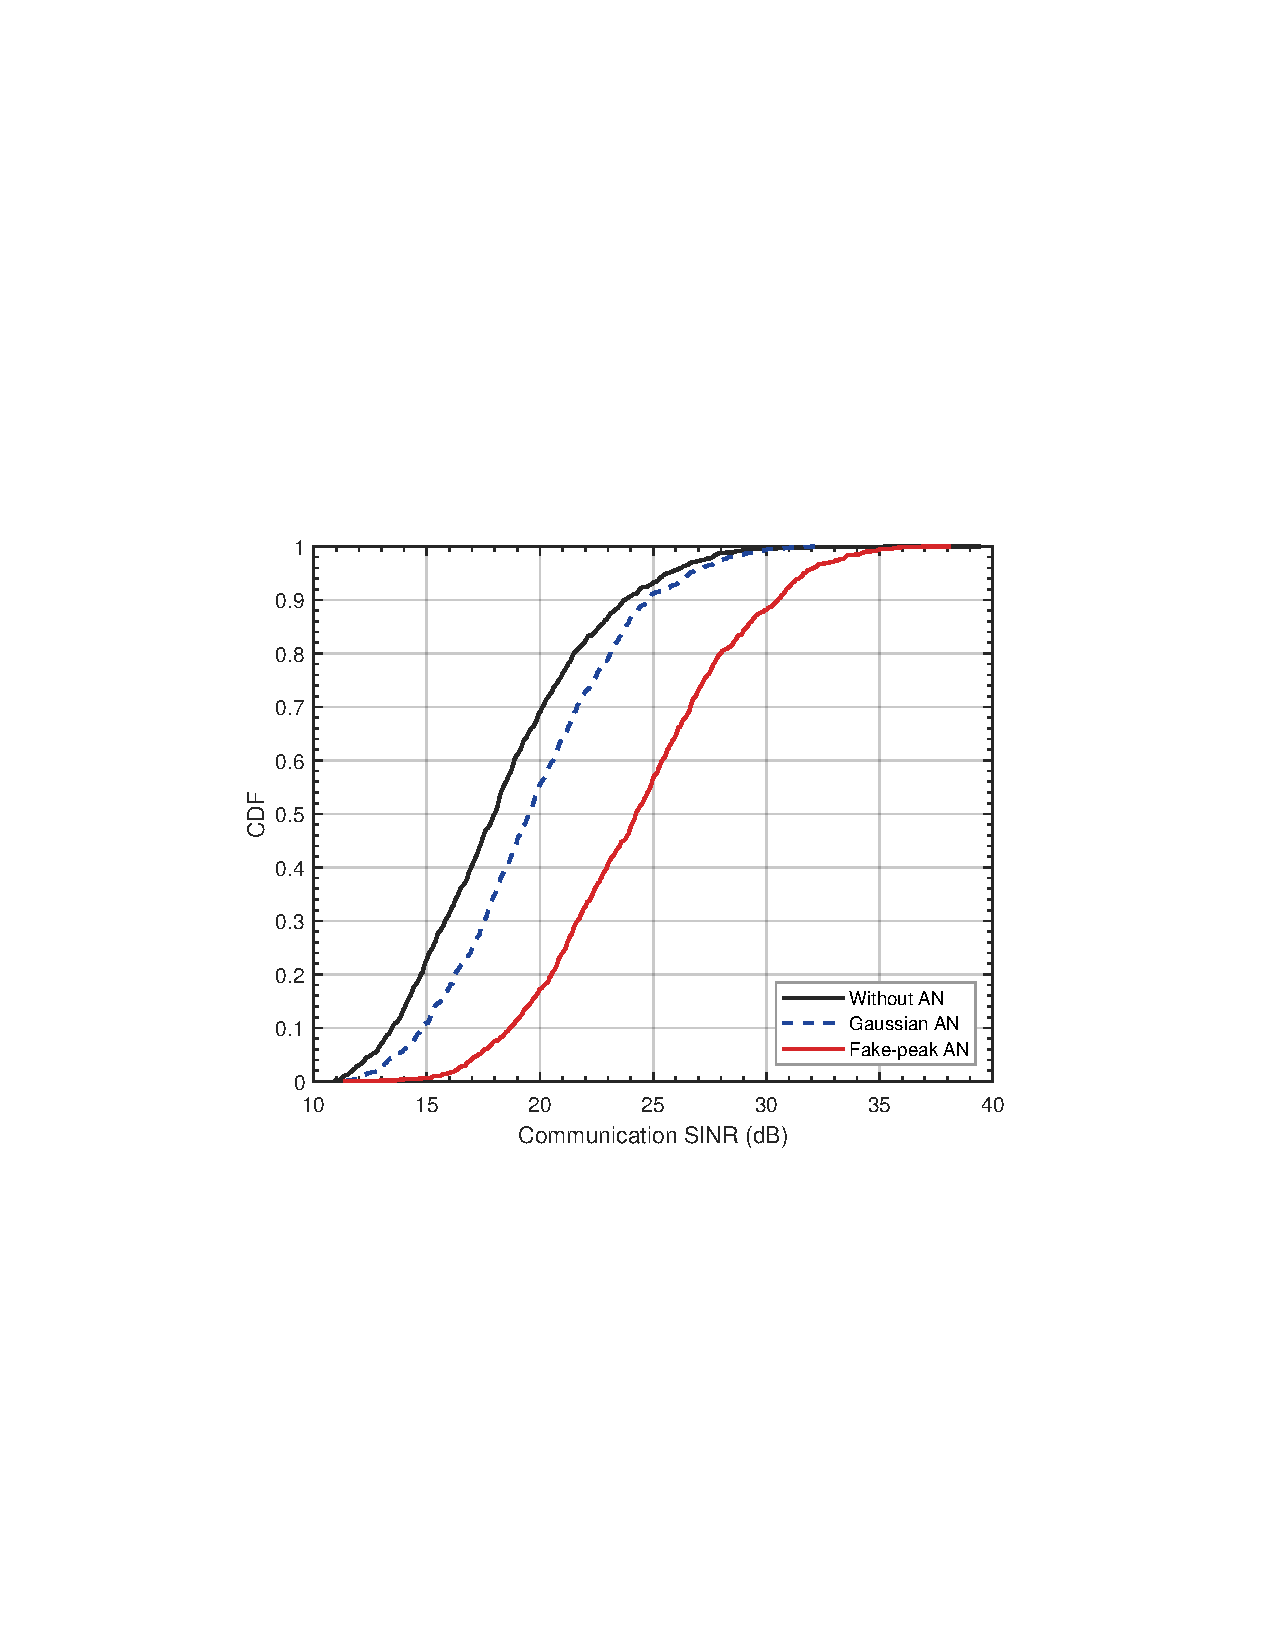
\includegraphics[width=0.8\columnwidth]{figure6.pdf}
    \caption{CDF of the minimum communication SINR under different AN designs.}
    \label{fig:sinr-cdf}
\end{figure}

Fig.~\ref{fig:sinr-cdf} further evaluates the communication-side impact by plotting the CDF of the minimum user SINR over all channel realizations. All three curves remain above the required $\Gamma_{\mathrm{comm}}=10$ dB threshold, confirming that the AN-aided designs preserve the communication QoS. The proposed fake-peak AN also yields a right-shifted SINR distribution, with the median minimum SINR increasing from about $18.0$ dB without AN to about $24.2$ dB. This indicates that the directional deception introduced for sensing privacy does not come at the expense of user reliability.



\section{Conclusion}
This letter proposed a fake-peak AN design against the internal beampattern-reconstruction attack in multi-static CF-mMIMO ISAC. By nulling AN on the receive-combiner-aware legitimate channel but leaving it visible to the raw-channel reconstruction process, the design steers a deceptive peak in a preset fake direction while preserving communication and sensing performance, and the joint problem is solved by a CCCP-MMSE alternating algorithm. Simulations show that the directional mutual information drops by roughly $3$ bits, the detection rate is markedly suppressed under both array sizes, and the sensing SNR is kept above $32$ dB. Extensions to imperfect-CSI robustness and multi-target settings are left for future work.


\bibliographystyle{IEEEtran}
\bibliography{references}

\end{document}
